\documentclass[11pt]{article}
\renewcommand{\baselinestretch}{1.8}
\usepackage{textcomp}
\usepackage{fontenc}
\usepackage{graphicx}
\usepackage{caption} % for Fig. captions
\usepackage{gensymb} % for \degree
\usepackage{placeins} % for \images
\usepackage[margin=1in]{geometry} % to set margins
\usepackage{setspace}
\usepackage{lineno}
%\usepackage{cite}
\usepackage{amssymb} % for math symbols
\usepackage{amsmath} % for aligning equations
\usepackage[sort&amp;compress]{natbib}
\usepackage{xr-hyper}
\externaldocument{diffsens_SUPP}

\bibliographystyle{..//..//sub_projs/refs/styles/newphyto.bst}

\linenumbers


\title{Differences in flower and leaf bud responses to the environment drive shifts in spring phenological sequences of temperate woody plants}\\

\date{}
\author{D.M. Buonaiuto $^{1,2,a}$, E.M. Wolkovich$^{3}$}

\begin{document}
\maketitle
\section*{Introduction}
\noindent One of the most widely documented biological effects of anthropogenic climate change are shifts in phenology, the timing of life cycle events, in plants \citep{Parmesan2003,Menzel2006,Cleland2007}. While phenology is generally advancing with climate change, the strength of these phenological shifts can vary substantially among specific phenological phases \citep{Augspurger:2020aa}. These differences alter the timing of phases relative to each other, changing the the duration of inter-phase periods that make up phenological sequences \citep{Ettinger2018}. Phenological sequences are a major driver of plant fitness that impact plant life history, resource allocation, demography and ecosystem processes \citep{Post:2008aa}. Shifts in phenological sequences will likely alter many of these processes, but the effects these shifts depend both on the direction (whether distinct phases are shifting closer together or farther apart) and magnitude (how much they are shifting relative to each other).\\ %EMWAug6: Nice!

\noindent Among deciduous woody plants, the relative timing of flower and leaf phenology, or flower-leaf sequences (FLSs), may be particularly consequential to fitness in temperate regions where flowering prior to leaf development is common \citep{Rathcke_1985,Gougherty2018}. %Long-term phenological observations over the last several decades indicate that, like other phenological sequences, FLSs are shifting due to anthropogenic climate change \citep{Buonaiuto2020} suggesting that some of the critical functions of FLSs may become compromised. However, observed FLS shifts vary among species, which may put some species at greater risk while benefiting others \citep{Buonaiuto2020}.\\  %EMWAug6: May need to inject a clause in the first few sentences of this paragraph to help readers along ...  maybe change "Long-term phenological observations over the last several decades indicate that, like other phenological sequences, FLSs are shifting due to anthropogenic climate change \citep{Buonaiuto2020} suggesting that some of the critical functions of FLSs may become compromised." to 
Long-term phenological observations over the last several decades indicate that, like other phenological sequences, FLSs are shifting due to anthropogenic climate change \citep{Buonaiuto2020}---for several species, the time between flowering and leafing appears to be increasing, but the strength of this trend varies among species and the direction of FLS shifts are not consistent across populations. These changes could affect the important functions of FLSs, which may put some species at greater risk while benefiting others.\\

\noindent Flowering before leaf development may be a critical adaptation for pollination efficiency in wind-pollinated taxa by eliminating pollen interception by the forest canopy \citep{Whitehead1969}. In insect-pollinated taxa, flowering-first may increase the visibility of flowers to pollinators \citep{Janzen1967,Savage2019}. Species with decreasing FLS interphases with climate change may experience increased pollen limitation as more wind pollen is intercepted by vegetative structures and flowers are obscured by developing leaves. Conversely, pollination efficiency could improve for species with lengthening FLS interphases (direction). A change in the FLS interphase of just a few days would likely have little impact on these processes, but if shifts were on the order of weeks, the impact on the pollination biology of a species could be highly significant (magnitude).\\

\noindent Predicting the direction and magnitude of any FLS shifts requires identifying the underlying mechanisms that drive the different responses to climate change among these phenophases for a diversity of woody plant species. %There is mounting evidence that plants respond more strongly to different environmental cues during different parts of their annual cycle. Cues use may vary among phenophases across the season because reliability of specific cues to indicate appropriate conditions changes over the season as well \citep{}. For example, woody plants rely more strongly on photoperiod as a cue for autumn phenological phases than for spring phases indicating that daylength is a more reliable cue for the cessation of growth than the start of growth\citep{}. However, this hypothesis does not explain different cue use among phenophases like spring flowering and leafing that occur close to each other in time under relatively similar conditions \citep{}.\\
Decades of research suggests that for woody plants in temperate regions, cool winter temperatures (chilling), warm spring temperatures (forcing) and day-length (photoperiod) are the primary drivers of both reproductive and vegetative phenology \citep{Forrest2010,Flynn2018}. However, observed FLS shifts indicate that there must be differences in how these cues influence phenological activity in floral and leaf buds. % but these differences have not been well characterized in wild species. 
Identifying these differences is a necessary step for predicting the direction and magnitude, and ultimately fitness impacts of FLS shifts with climate change.\\
 
\noindent Studies that have attempted to identify the differences between reproductive and vegetative phenology in woody plants have mostly focused on crop species and two common, yet competing, explainations have emerged:\\

%\noindent What we call the \textbf{precocity hierarchy hypothesis (PHH)} suggests that reproductive and vegetative buds respond similarly to most environmental cues, but have consistently different forcing requirements for the commencement of phenological activity \citep{Guo_2014,COSMULESCU:2020aa,Cosmulescu:2018aa}.  \\%EMWAug6: I would name the hypotheses after you introduce them ... some possible edits also:
% What we call the \textbf{precocity hierarchy hypothesis (PHH)} suggests that reproductive and vegetative buds respond similarly to most environmental cues, but have consistently different forcing requirements for the commencement of phenological activity --> 
\noindent One hypothesis suggests that reproductive and vegetative buds utalize the same underlying enviromental cues, but have different threshold responses to forcing, with whichever bud type bursts later---leaves or flowers---having a higher threshold \citep{Guo2014,COSMULESCU:2020aa,Cosmulescu:2018aa}. Under this hypothesis, which we call the precocity hierarchy hypothesis (PHH), leaf and flower buds share the same suite of cues and develop similarly to non-forcing cues but they differ in the thermal units required for budburst.\\

\noindent By contrast, an alternative hypothesis suggests that flower and leaf buds differ in the strength of their phenological responses to the multiple environmental cues \citep{Citadin2001,Gariglio2006,Aslani2009,Mehlenbacher:1991aa}. Under this hypothesis, which we call the differential sensitivity hypothesis (DSH), despite the fact that leaf and flower buds are exposed to similar environmental conditions, each bud type may rely more or less on certain cues, producing different and variable phenological patterns.\\

\noindent While these mechanisms may produce similar phenological patterns under historic climate conditions, they have different implications regarding the potential for FLS shifts with climate change. The PHH suggests that FLS variation is largely a product of climate variation during the interphase. If spring temperatures increase with climate change, the second phenophase of the FLS with be accelerated relative to the first and the FLS interphases will decrease, but given the relative auto-correlation of spring temperatures \citep{Di-Cecco:2018aa}, these shifts should be relatively muted. \\

\noindent The DSH suggests that with significant cue use differences among bud types, there will be strongly localized effects of climate change on FLSs. Shifts in FLS variation will depend on the direction and rate of change in cues at specific locations and the differential sensitivity of reproductive and vegetative phenology to cue combinations. This hypothesis allows not only for larger magnitude shift in FLSs, it also suggest that the magnitude of shifts may be highly divergent among populations of the same species.\\

%\noindent Simple simulations suggest that each mechanism will produce different, recognizable signatures for phenological patterns under experimental conditions. For the precocity hierarchy \\

\noindent In this study we test these hypotheses by observing phenological responses to changing environmental conditions for both flower and leaf buds for a suite of temperate shrubs and trees. We subjected dormant twig cuttings of 10 species to multiple levels of forcing, chilling and photoperiod treaments in growth chambers and compared flower and leaf phenological responses to environmental change using a Bayesian hierarchical modeling approach. We then leveraged these data to to make generalized projections for how FLSs may shift with climate change and identify avenues for further research.\\ 

\section*{Methods}

\subsection*{Growth chamber study}
\noindent We sampled all plant material used in this experiment from Harvard Forest in Petersham, MA. On October 25, 2016, immediately after most plants in the area entered dormancy but before they could accumulate any significant chilling in the field,  we collected branch cuttings from 7-13 individuals of 12 woody plant species (4-12 cutting per individual for a total of 48-56 per species). The species consisted of a mix of deciduous shrubs, understory and canopy trees commonly found in mesic hardwood forests of the eastern United States (see tab. \ref{tab:splist} for species list). We transported all cuttings to the Arnold Arboretum in Boston, MA where they were re-cut in water to prevent callousing and cavitation and placed in 500 ml Erlenmeyer flasks with distilled water.\\ 

\noindent We randomly assigned cuttings to a full set of eight experimental treatments; two levels of chilling (4 vs 8 weeks at 4\degree C), two levels of temperature (24\degree C:18\degree C (day/night) warm vs 18\degree:12\degree C (day/night) cool) and two levels of photoperiod (12 vs 8 hours). We alternated day/night temperature periodicity on a 12 hour schedule to reduce co-variation with photoperiodicty. We re-cut all twig and changed the water every 7-10 days and rotated all treatments between growth chambers every two weeks to minimize chamber effects. We made phenological observations every 2-3 days using a modified BBCH scale for woody plants \citep{Finn2007} for three month following release from chilling conditions. In this period we assess three phenological phases: budbreak (BBCH phase 07), leaf unfolding (BBCH phase 15) and first flower open (BBCH 60). At the conclusion of this period we assessed all individuals that did not undergo budbreak and excluded any dead individuals for analysis.

\subsection*{Data analysis}
\noindent To assess the sensitivity of each phase, we fit mixed-effect hierarchical models with chilling, forcing, photoperiod and all two-way interactions as the fixed effects and species as a grouping factor on both the slopes and the intercepts. We chose a Bayesian, hierarchical approach in order to identify systematic trends across species' responses while accounting for sample size, variance and the unique effect of each species. Two species \textit{Betula allegheniensis} and \textit{Acer saccharum} produced no flowers in our trial, so we excluded them from our analysis.\\

%emw8May2020: I think we can cut the below paragraph, as long as we specify the intercept condition in the captions (more useful to specify it there anyway); likewise use of dummy variables should be obvious when looking at model output and figures as long as clearly labeled (e.g., 4 hour difference) 
%\noindent Because we applied two levels for each environmental treatment in the experiment, we re-coded each treatment as 0/1 dummy variables to improve model performance, so model intercepts can be interpreted as the predicted phenological response when all treatments are at their lowest level. Given that true zeros for these treatment levels are unrealistic in nature, in addition to computational efficiency, this approach also allows for a realistic interpretation of model intercepts.\\  


We modeled the effects of environmental parameters on flower opening and leaf budburst separately.
We also fit a model with FLS interphase (day of budburst- day of flowering) as a response variable to compare these estimates with field observations.\\

The models we fit appear below:\\

$y_{[i]} \sim N(\alpha_{sp_{[i]}}+\beta_{forcing_{sp[i]}}+\beta_{chilling_{sp[i]}}+\beta_{photoperiod_{sp[i]}}+\beta_{forcing x chilling_{sp[i]}}+\beta_{forcing x photoperiod_{sp[i]}}+\beta_{chilling x photoperiod_{sp[i]}})$\\

Where $y_{[i]}$ is either the day of the experiment leaf budburst, day of first flower opening or FLS interphase length.  We modeled the $\alpha$ and each $\beta$ parameter at the species level using the formula:\\

$\alpha_{x_{sp}} $or $\beta_{x_{sp}} \sim N(\mu_x,\sigma^2_x)$\\

\noindent We fit all models using the R package ``brms" \citep{Burkner2018}. We ran each model on four chains with 4000 iterations with a 3000 iteration warm up for a total of 4000 sampling iterations. In both models we used weakly informative priors and increasing the priors 5-fold did not affect the model results.\\


\subsection*{Climate change predictions}
\noindent To apply our model results to general climate change projections we chose our environmental treatments in this experiment to broadly reflect historic and future conditions at our sampling site. Our low forcing treatment approximated average spring temperature (March/April) at the site while our high temperature treatment reflects a 5 \degree C increase. Average field chilling (calculated from 15 Oct - 15 April, measured in Utah units) at Harvard Forest is 979.64, approximately 60\% of the difference between our low and high chilling treatment (Fig. \ref{tab:chillcomps}). Thus, our low chilling treatment represents a feasible estimate for a decrease in chilling with climate change and our high chilling treatment approximate reasonable increase. We should note that our low photoperiod treatment (8 hours of daylight) is well below the photoperiod experienced at Harvard Forest, but given that the photoperiod effects are expected to be small, we chose more extreme values in order to robustly estimate an effect (i.e., increasing statistical power). For this reason, our climate change projections for FLS variation are based on our high photoperiod treatment alone.\\

\noindent We used our flower and budburst models to project for each species in our study:\\
\begin{enumerate}
\item FLSs under average environmental conditions  (treatments: low forcing, ~6.5 weeks of chilling treatment)
\item FLS shifts with spring warming only (high forcing, ~6.5 weeks of chilling treatment)
\item FLS shifts with warming and increased chilling ((high forcing, ~8 weeks of chilling treatment)
\item FLS shifts with warming and decreased chilling ((high forcing, ~4 weeks of chilling treatment)

\end{enumerate}

\noindent To validate our predictions, we compared our FLS interphase model estimates of ``average" condition FLS interphases to long term phenological records from Harvard Forest \citep{OKeefe2015} for five species common to both datasets (Fig. \ref{fig:validate}), and found them to be comparable. Given the variable dynamics of shifts in environmental forcing and chilling with climate change over time and space, these projections should not be treated as absolute predictions of the magnitude of FLS shifts with climate change. Instead, we provide these projections to identify general trends in how FLSs could shift with warming and demonstrate the range of possibilities vary based on individual characteristics of plant species and the specific climate dynamics.\\

\section*{Results}
\subsection*{Growth chamber study}
\noindent  Both flower and leaf buds advanced with higher forcing and longer chilling duration (flowers: 21 day advance/\delta chilling duration, 18 day advance/\delta forcing temperature, leaves: 30 day advance/\delta chilling, 17 day advance \delta forcing) , but increases in both of these cues together offset these advances as seen in the delaying effect of their interaction ( by 6 and 12 days for flowers and leaves respectively) (Fig. \ref{fig:model},Tab. \ref{tab:modelests}). Leaf and flower buds diverged in their responses to increasing photoperiod, with flower phenology advancing and leaf phenology being delayed when the other two cues were at low levels (Fig. \ref{fig:model}, Tab. \ref{tab:modelests}). As seen in the interactions between photoperiod and chilling and photoperiod and forcing, increasing chilling or forcing with longer photoperiod advanced the phenology of both bud types. For both bud types, chilling and forcing were the dominant cues, while increasing photoperiod produced a more muted phenological response (Fig. \ref{fig:model}). \\

\noindent While leaf and flower bud phenological responses to environmental cues were qualitatively similar, the strength of their responses to each cue differed substantially. Leaf buds responded more strongly to chilling than flower buds ( 1.4x ) , and had a stronger response to all cue interactions(forcing:chilling 2x, photoperiod:chilling 7.1x, photoperiod:forcing 2.4x) (Fig. \ref{fig:model}Tab. \ref{tab:modelests}). Across all species both bud types displayed a relatively proportionate response to forcing (18 and 17 day advance for flower and leaves respectively) (Fig. \ref{fig:model}, Tab. \ref{tab:modelests}). While there was significant variation among species in their strength of their response to forcing between bud types, no species displayed the characteristic sensitivity pattern of the PHH in which the sensitivity to forcing of the second phase twice as strong as the sensitivity of the first phase (simulations for supp?). Rather, the differences in the strength of the responses of each bud type to each environmental cue combination is signature of the DSH.\\

    \subsection*{Climate change predictions}
\noindent Our model predicted that both flower and leaf phenology will advance in most of our generalized scenarios for most species, but shifts in FLS depended strongly on how forcing levels change relative to chilling duration (Fig. \ref{fig:preddy}). Following the significant differences in sensitivity to chilling between flowering and leafing phenology we found in our model, FLS interphases were more strongly influenced by changes in chilling exposure than increased forcing alone. The direction and magnitude of shifts in FLS interphases depended on species and the specifics of FLS phase order, with flowering-first and flowering-concurrently species tending to show more profound alterations to FLS patterns than leafing-first taxa. Under some warming scenarios, our model predicted that  FLS interphases for some species may effectively disappear or the order of phenophases in the FLS may switch (Fig. \ref{fig:preddy}).


\section*{Discussion}
\noindent In our study, variation in FLS patterns of deciduous woody plants across environmental conditions was dictated by differences in the strength of the response of flower and leaf buds to the primary environmental cues of spring phenology, with differences in the chilling response among bud types being the strongest driver of FLS variation. These results together suggest that climate change has potential to signifiantly disrupt FLSs as global warming alters historic chilling patterns across the temperate zone. Across all of our treatment combinations, species differed in their differential sensitivity to environmental cues, but under our high chilling treatment, which approximated the historic chilling durations at our collection site, the FLSs for most species followed the predicted pattern of the PHH, with the sensitivity of the second phase of the FLS to forcing approximately twice as strong as that of the first phase \ref{fig:phh}. This may explain why the two FLS hypotheses have been difficult to distinguish under current field conditions where in most locations chilling requirements for both bud type were frequently met under historic climate conditons \citep{}. With site-specific FLS shifts, species-specific FLS functions, and this difficultly of assessing differential sensitivity in the field there is a need for generalizing principles from experimental studies such as this one, to more fully anticipate the implications of FLS shifts and focus research efforts to the species that may be most affected by FLS shifts with climate change.

\subsection*{Implications of the DSH for FLS shifts with climate change} %maybe need to make this section longer 
The strong differential sensitivity to chilling between flower and leaf buds we found in our study suggests complex FLS dynamics with climate change. Predicted shifts in chilling are highly variable across both time and space-- because chilling only accumulates at intermediately low temperatures warming may increase chilling at some locations while decreasing it in others \citep{}. This suggests that the direction and magnitude of FLS shifts is likely to vary substantially among populations based on the specific cue combinations at a given locality. Long-term phenology records show there was already substantial intra-specific variation in FLSs at the population level \citep{Buonaiuto2020} and our findings suggest that these populations level differences may be further amplified by climate change.\\

Increased population level heterogineity of in FLSs has potential to alter patterns of pollen disperal and gene flow across the landscape \citep{}. For example, advancing canopy closure relative to flowering impedes long-distance pollen transport \citep{Mileron2012}. With divergent FLS shifts at the population level, sires from populations in which climate dynamics are extending FLS interphases may increase their contribution landscape patterns of gene flow relative to populations in which FLSs are reduced. Depending on the spatial arrangement of these populations and other factors such as pollinator movement or previaling wind direcitons, this could either facilitate or impeded genetic rescue of climate stressed populations \citep{}.

Despite these theoretical implications, there is currently little empirical scholarship regarding how inter-population variation in FLS patterns may impact landscape processes like gene flow and recruitment. Our study offers several insights as to why this must be the case. \\

\subsection{Differential sensitivity in the field}

\subsection{Gernalizing principle for species-specific response}

First, we demostrated that if chilling is met the patterns appear in the PHH, this trend is also apparent in field based studies, so the magnitidue of potential for shifts and in general and certainly at the population level wasn't always so apparent.\\

Second, both direction and magnitide of FLSs  species specific. For example

If FLS shifts are difficult to detect in the field and must have different trends and implications for indivudal species it will be very difficult to assess.

\subsection*{Patterned responses}


%\subsection*{Differential sensitivity to environmental cues}
%\noindent The results of our experiment suggest that the relative timing of the component phases of flower-leaf sequences in deciduous, woody plants is structured by differences in the strength of the response of each bud type to the primary environmental cues of spring phenology. Specifically, vegetative buds were more sensitive to chilling and flower buds more sensitive to photoperiod. The sensitivity of flower and leaf buds to changes in forcing were proportionate in magnitude, but interactions between forcing and the other two cues drove a stronger response in leaf buds than flower buds. Together, the phenological response patterns we observed are more closely aligned with the predictions of the DSH than the PHH. Our results suggest that differential sensitivity to the environment among flower and leaf buds generates the high level of inter-annual FLS variation observed in nature, and will dictate the direction and magnitude of FLS shifts with climate change.\\.

%\noindent While both flower and leaf bud phenology advanced with increasing chilling duration, the sensitivity of the response to chilling was greater in leaf buds. This result is consistent with experimental manipulations of tree-crop phenology which also found a higher sensitivity to chilling for leaf buds \citep{Gariglio2006,Citadin2001}. We found that floral phenology was more tightly linked to changes in photoperiod than leaf phenology. While we found no literature that evaluated the differential sensitivity of flower and leaf buds to photoperiod, our findings are consistent with genetic work in the model genus \textit{Populus} suggests that flowering may be under stronger photoperiodic control that leafing \citep{}.\\

%\noindent Our results failed to support the PHH, but the patterns of phenological responses in our study may reveal key insights as to why this hypothesis may be so prevalent in the literature. We found that when we subset our data to include only high chilling and photoperiod treatments, the sensitivity of flower and leaf buds to forcing matched the predicted pattern of the PHH with the second phase of the phenological sequence demonstrating approximately twice the sensitivity of the first phase for many of these species of our studies (Fig. \ref{fig:phh}). This suggest that when chilling and photoperiod requirements are met, differences in the heat threshold requirements between flower and leaf buds structure FLSs.\\

%\noindent If under historic climate conditions the chilling requirement of most species was generally met in the field our results predict that the resulting FLS pattern would reflect a precocity hierarchy, and several of the studies that found support for the PHH are based on field observations \citep[e.g.][]{Guo2014,COSMULESCU:2020aa}. However, as winter temperature continue to change with global warming, it is likely that the regional chilling patterns will be disruption and the differential sensitivity of flower and leaf buds to the environment will have more pronounced effects on FLS patterns.

%\subsection*{FLS shifts with climate change}
%\noindent The support we found for the DSH in our study suggests that the direction and magnitude of FLS shifts with climate change will depend on how cues at a given location change relative to each other. We found that changes in the chilling cue strongly amplified the differential sensitivity of bud types to the environment, suggesting that this cue may drive FLS shifts with climate change. Because chilling only accumulates at intermediately low temperatures, warming may increase chilling at some locations while decreasing it in others \citep{}. This suggests that the direction and magnitude of FLS shifts is likely to vary substantially among populations based on the specific cue combinations at a given locality. Long-term phenology records show there was already substantial intra-specific variation in FLSs at the population level \citep{Buonaiuto2020} and our findings suggest that these populations level differences may be further amplified by climate change. There is currently little scholarship regarding how inter-population variation in FLS patterns may impact landscape processes like gene flow and dispersal, but given the hypothesized contribution of FLSs to reproductive fitness, this should remain an active area of research inquiry.\\

%\noindent Despite the fact that in our experiment we found photoperiod to be an important cue dictating FLS shifts, we modeled climate change scenarios with a constant photoperiod in our FLS projections with climate change. Climate change does not directly impact photoperiod, but warming does shift the time of year when plants become phenologically active, changing the photoperiod they experience. However, depending on the latitude, phenology would have to shifts by at minimum several weeks before the experience photoperiod would change substantially \citep{Ettinger}. However, at high latitudes where photoperiod changes more rapidly over the season, the experienced photoperiod may mute the FLS shifts captured in our projections. This may be particularly important as species shift shift their distribution pole ward with climate change and begin to encounter novel photoperiod regimes \citep{WAY:2015aa}.\\

%\noindent An additional complicating factor in predicting FLS shifts with climate change is that our experimental results and climate change projections suggest that species will differ in the direction and magnitude of their FLS shifts. Several species, \textit{Acer rubrum} ,\textit{Ilex verticillata}, \textit{Prunus pensylvanicum}, \textit{Prunus virginiana}, and \textit{Viburnum acerifolium}, had FLSs that were relatively robust to changing environments. For other species, \textit{Acer pensylvanicum}, \textit{Vaccinium corymbosum} and \textit{Ilex mucronata}, which typically begin to produce leaves shortly before flowers open, projected FLS shifts were moderate, with the combination of increased forcing coupled with a reduction in chilling driving the strongest shifts in FLSs. The two species with the most significant FLS shifts across treatment combinations and climate change projections were \textit{Comptonia peregrina} and \textit{Corylus cornuta} (Fig. \ref{fig:preddy}). In all of our climate change scenarios, the FLS interphase was dramatically reduced in these taxa.\\ 

%\noindent It is likely that these three difference response patterns we observed correlate to broader anatomical, physiological and phenological differences among species. We did not have the taxonomic resolution in this study to conclusively identify and character traits that may correlate with FLS shifts, but we observed some general patterns that may sever as starting hypotheses for future inquiry in this area.\\

%\noindent The species that maintained FLS structure across climate change scenarios generally shared a strongly leafing-first FLS, with a fairly long FLS interphase. These species tended to have mixed buds so there may be strong physical constraints on their FLSs. By contrast, the species that were most sensitive to FLS shifts were monoecious, flowering-first, wind-pollinated shrubs. This result may reflect other evidence that wind-pollinated species appear to be more sensitive to climate change than biotically pollinated taxa \citep{Ziello:2012aa}. Given the hypothesized function of FLS in wind-pollinated species, the direction and magnitude of FLS shifts we observed could suggest that that these species, and flowering-first, wind-pollinated taxa in general, may face particular risk for reproductive performance reductions. 

%\noindent Much of the conversation around phenology and pollination in the context of global change has centered around trophic mismatches between pollinator and floral phenology \citep{Memmott2007}, which is of little relevance to abiotically pollinated taxa. By contrast, the possibility that the effect of FLS shifts with climate change may be particularly important for abiotically pollinated woody plants and the scope and impact of FLS shifts in these taxa suggest they should be explored in greater detail in the future.\\

\section*{Conclusion:}
\noindent Our experiment provides strong evidence that while flower and leaf buds respond to the same suite of environmental cues to initiate spring phenological activity, the different bud types rely on each cue with differing strength. This differential sensitivity to cues drives variation in flower-leaf sequences and will dictate the magnitude and direction of FLS shifts with climate change. Shifts in FLSs with climate change are likely to vary across forest communities and depend on the specific combinations of cue levels at a given locality and the species represented there. More research is needed to identify species' traits that may correlate with the potential for FLS shifts and to understand the fitness implications of FLS shifts.

\bibliography{..//..//sub_projs/refs/hyst_outline.bib} 

\section*{Tables}
\begin{table}[ht]
\centering
\begin{tabular}{|r|r|r|r|r|r|}
  \hline
 & Estimate & Est.Error & Q25 & Q75 & phase \\ 
  \hline
Intercept & 77.54 & 10.01 & 70.91 & 84.01 & flower \\ 
 & 70.30 & 8.93 & 64.56 & 76.01 & budburst \\ 
  \hline
  Chill & -21.31 & 7.54 & -26.14 & -16.78 & flower\\ 
   & -30.35 & 5.20 & -33.66 & -27.06 & budburst\\ 
 \hline
  Light & -5.99 & 5.83 & -9.73 & -2.12 & flower\\ 
   & 5.95 & 5.12 & 2.68 & 9.29 & budburst\\ 
  \hline
  Force & -18.87 & 6.36 & -22.85 & -14.85 & flower\\ 
 & -17.39 & 5.16 & -20.70 & -14.01 & budburst \\ 
  \hline
  Chill:Light & -0.70 & 6.17 & -4.60 & 3.44 & flower\\ 
     & -5.04 & 4.16 & -7.73 & -2.26 & budburst\\ 
  \hline
  Chill:Force & 6.75 & 6.62 & 2.73 & 10.96 & flower \\ 
   & 12.31 & 4.77 & 9.28 & 15.42 & budburst \\ 
  \hline
  Light:Force & -5.42 & 6.22 & -9.39 & -1.30 & flower \\ 
    & -12.90 & 4.12 & -15.54 & -10.17 & budburst\\ 
   \hline
\end{tabular}
\label{tab:modelests}
\caption{\textbf{Model estimates of the effect of variation in chilling, forcing and photoperiod on the flower and leaf phenology of 10 temperate woody plant species suggest that the strength of phenological responses to environmental change is phase specific.} }
\end{table}






   \hline
\end{tabular}
\end{table}
\section*{Figures}

\begin{figure}[h!]
    \centering
         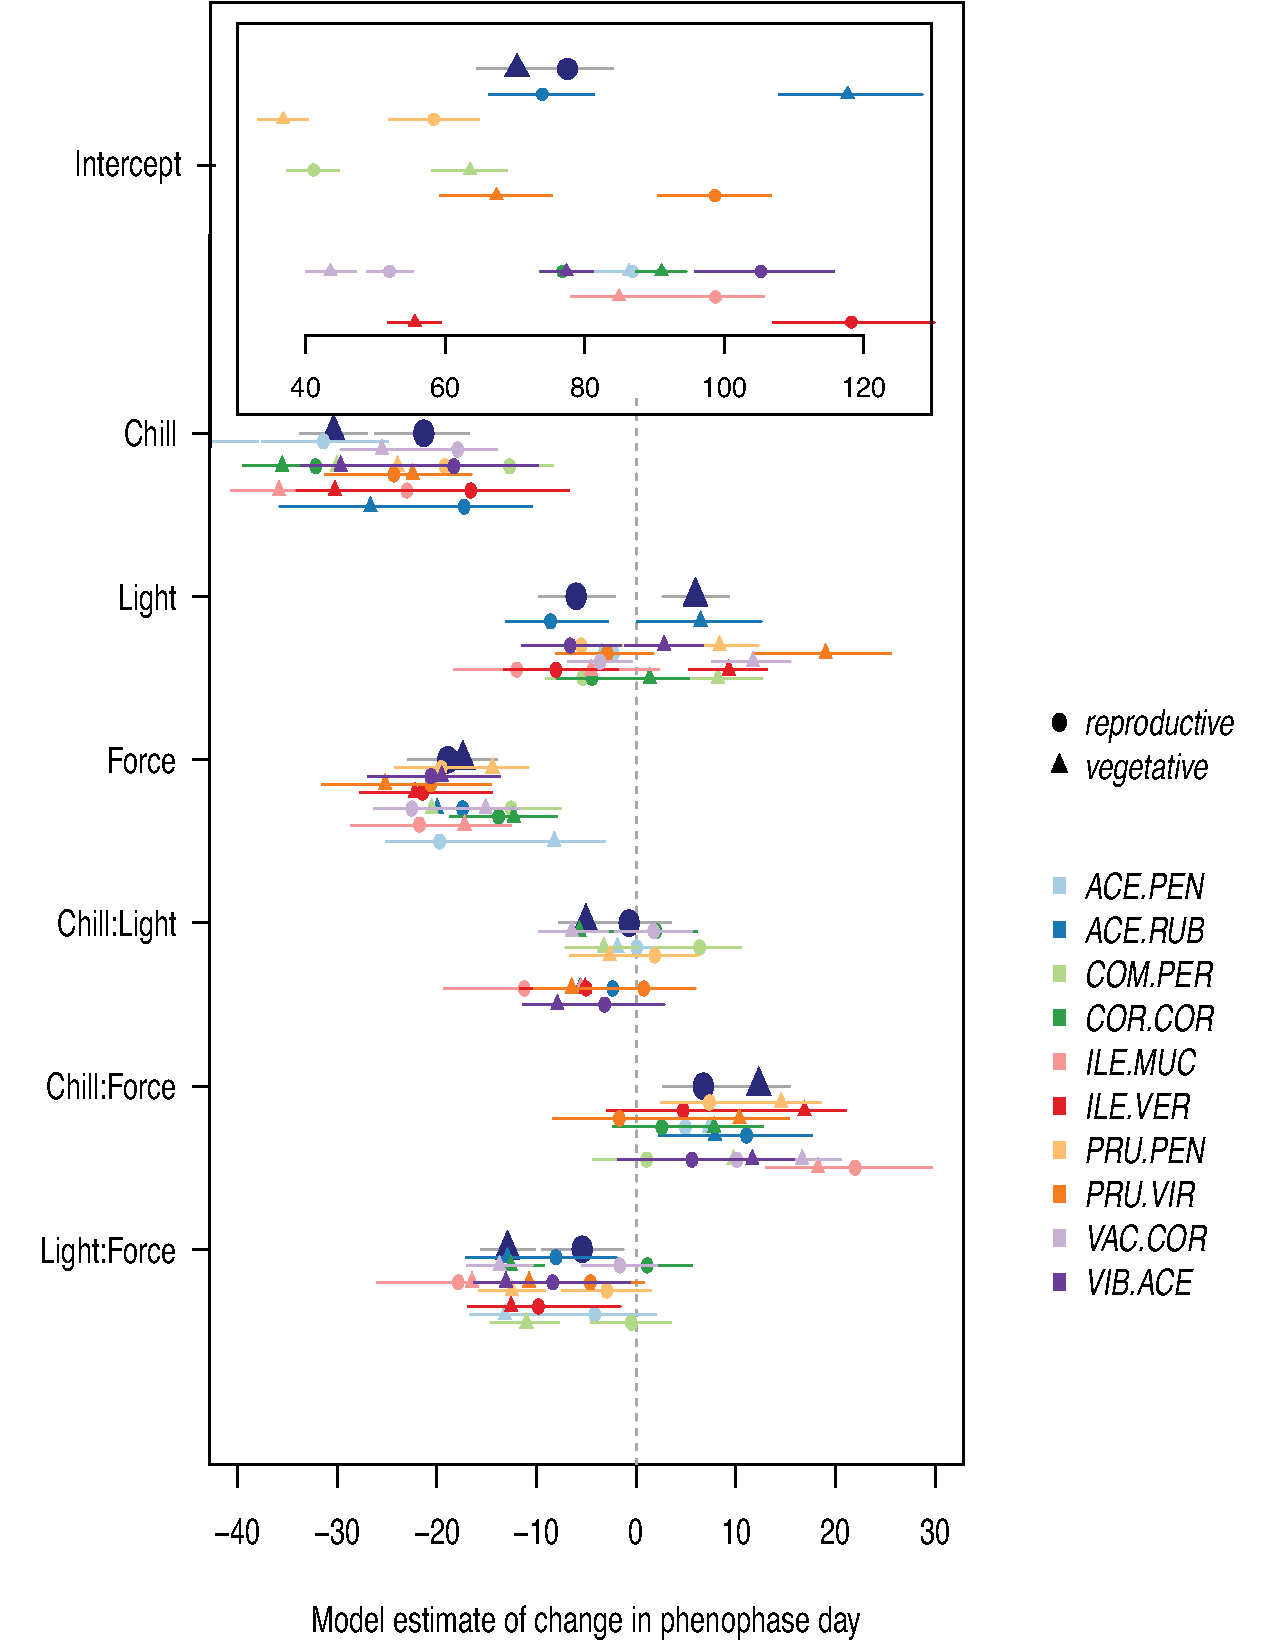
\includegraphics[width=\textwidth]{..//Plots/Flobuds_manuscript_figs/budburstvsflowering.pdf}
    \caption{\textbf{Experimental results suggest differential sensitivity to environmental cues between flower and leaf buds}. Vegetative buds (circles) as more sensitive to chilling and interaction between chilling and forcing. Flower buds (triangles) advance with photoperiod increases but leaf buds appear to delay. These differential sensitivities dictate how FLS patterns vary with changing environmental conditions.}
    \label{fig:model}
\end{figure}

\begin{figure}[h!]
    \centering
         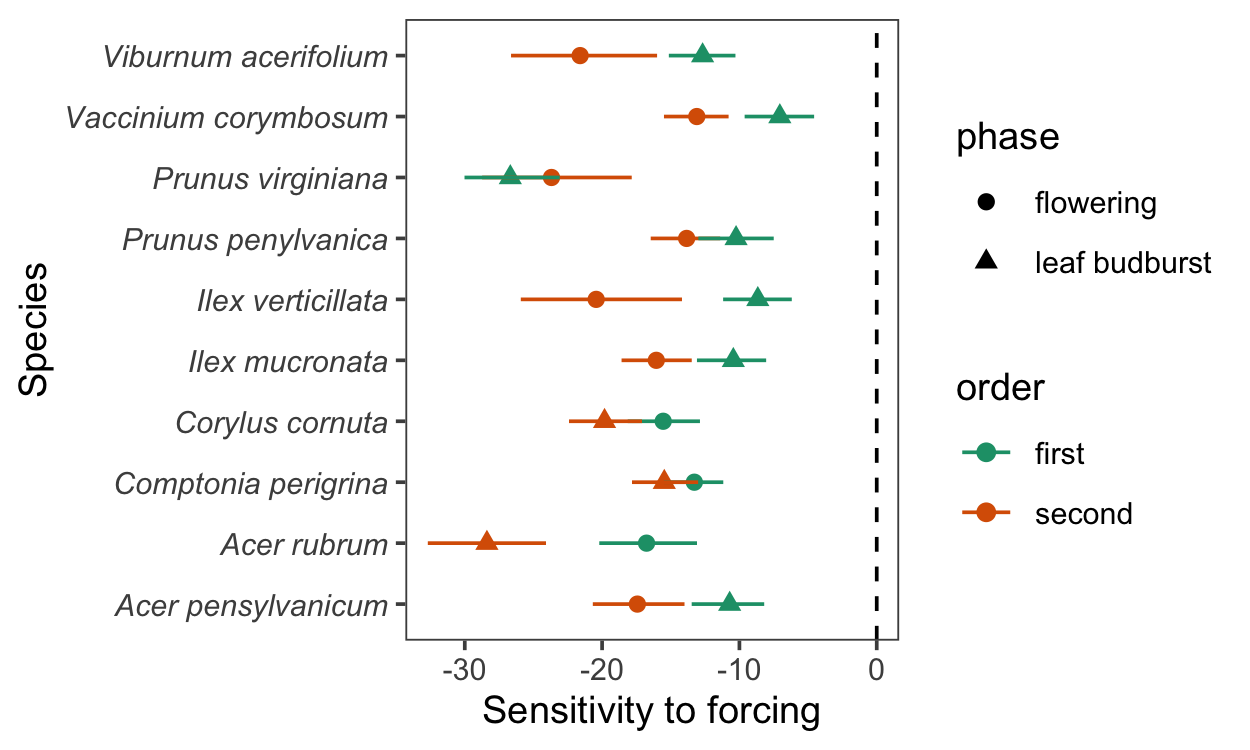
\includegraphics[width=\textwidth]{..//Plots/Flobuds_manuscript_figs/phh_plot.png}
    \caption{\textbf{With high chilling and photoperiod, the comparative response to forcing  among leaf and flower buds resemble patterns predicted by the precocity hierarchy hypothesis (PHH)} Say a bit more about this.}
    \label{fig:phh}
\end{figure}

\begin{figure}[h!]
    \centering
 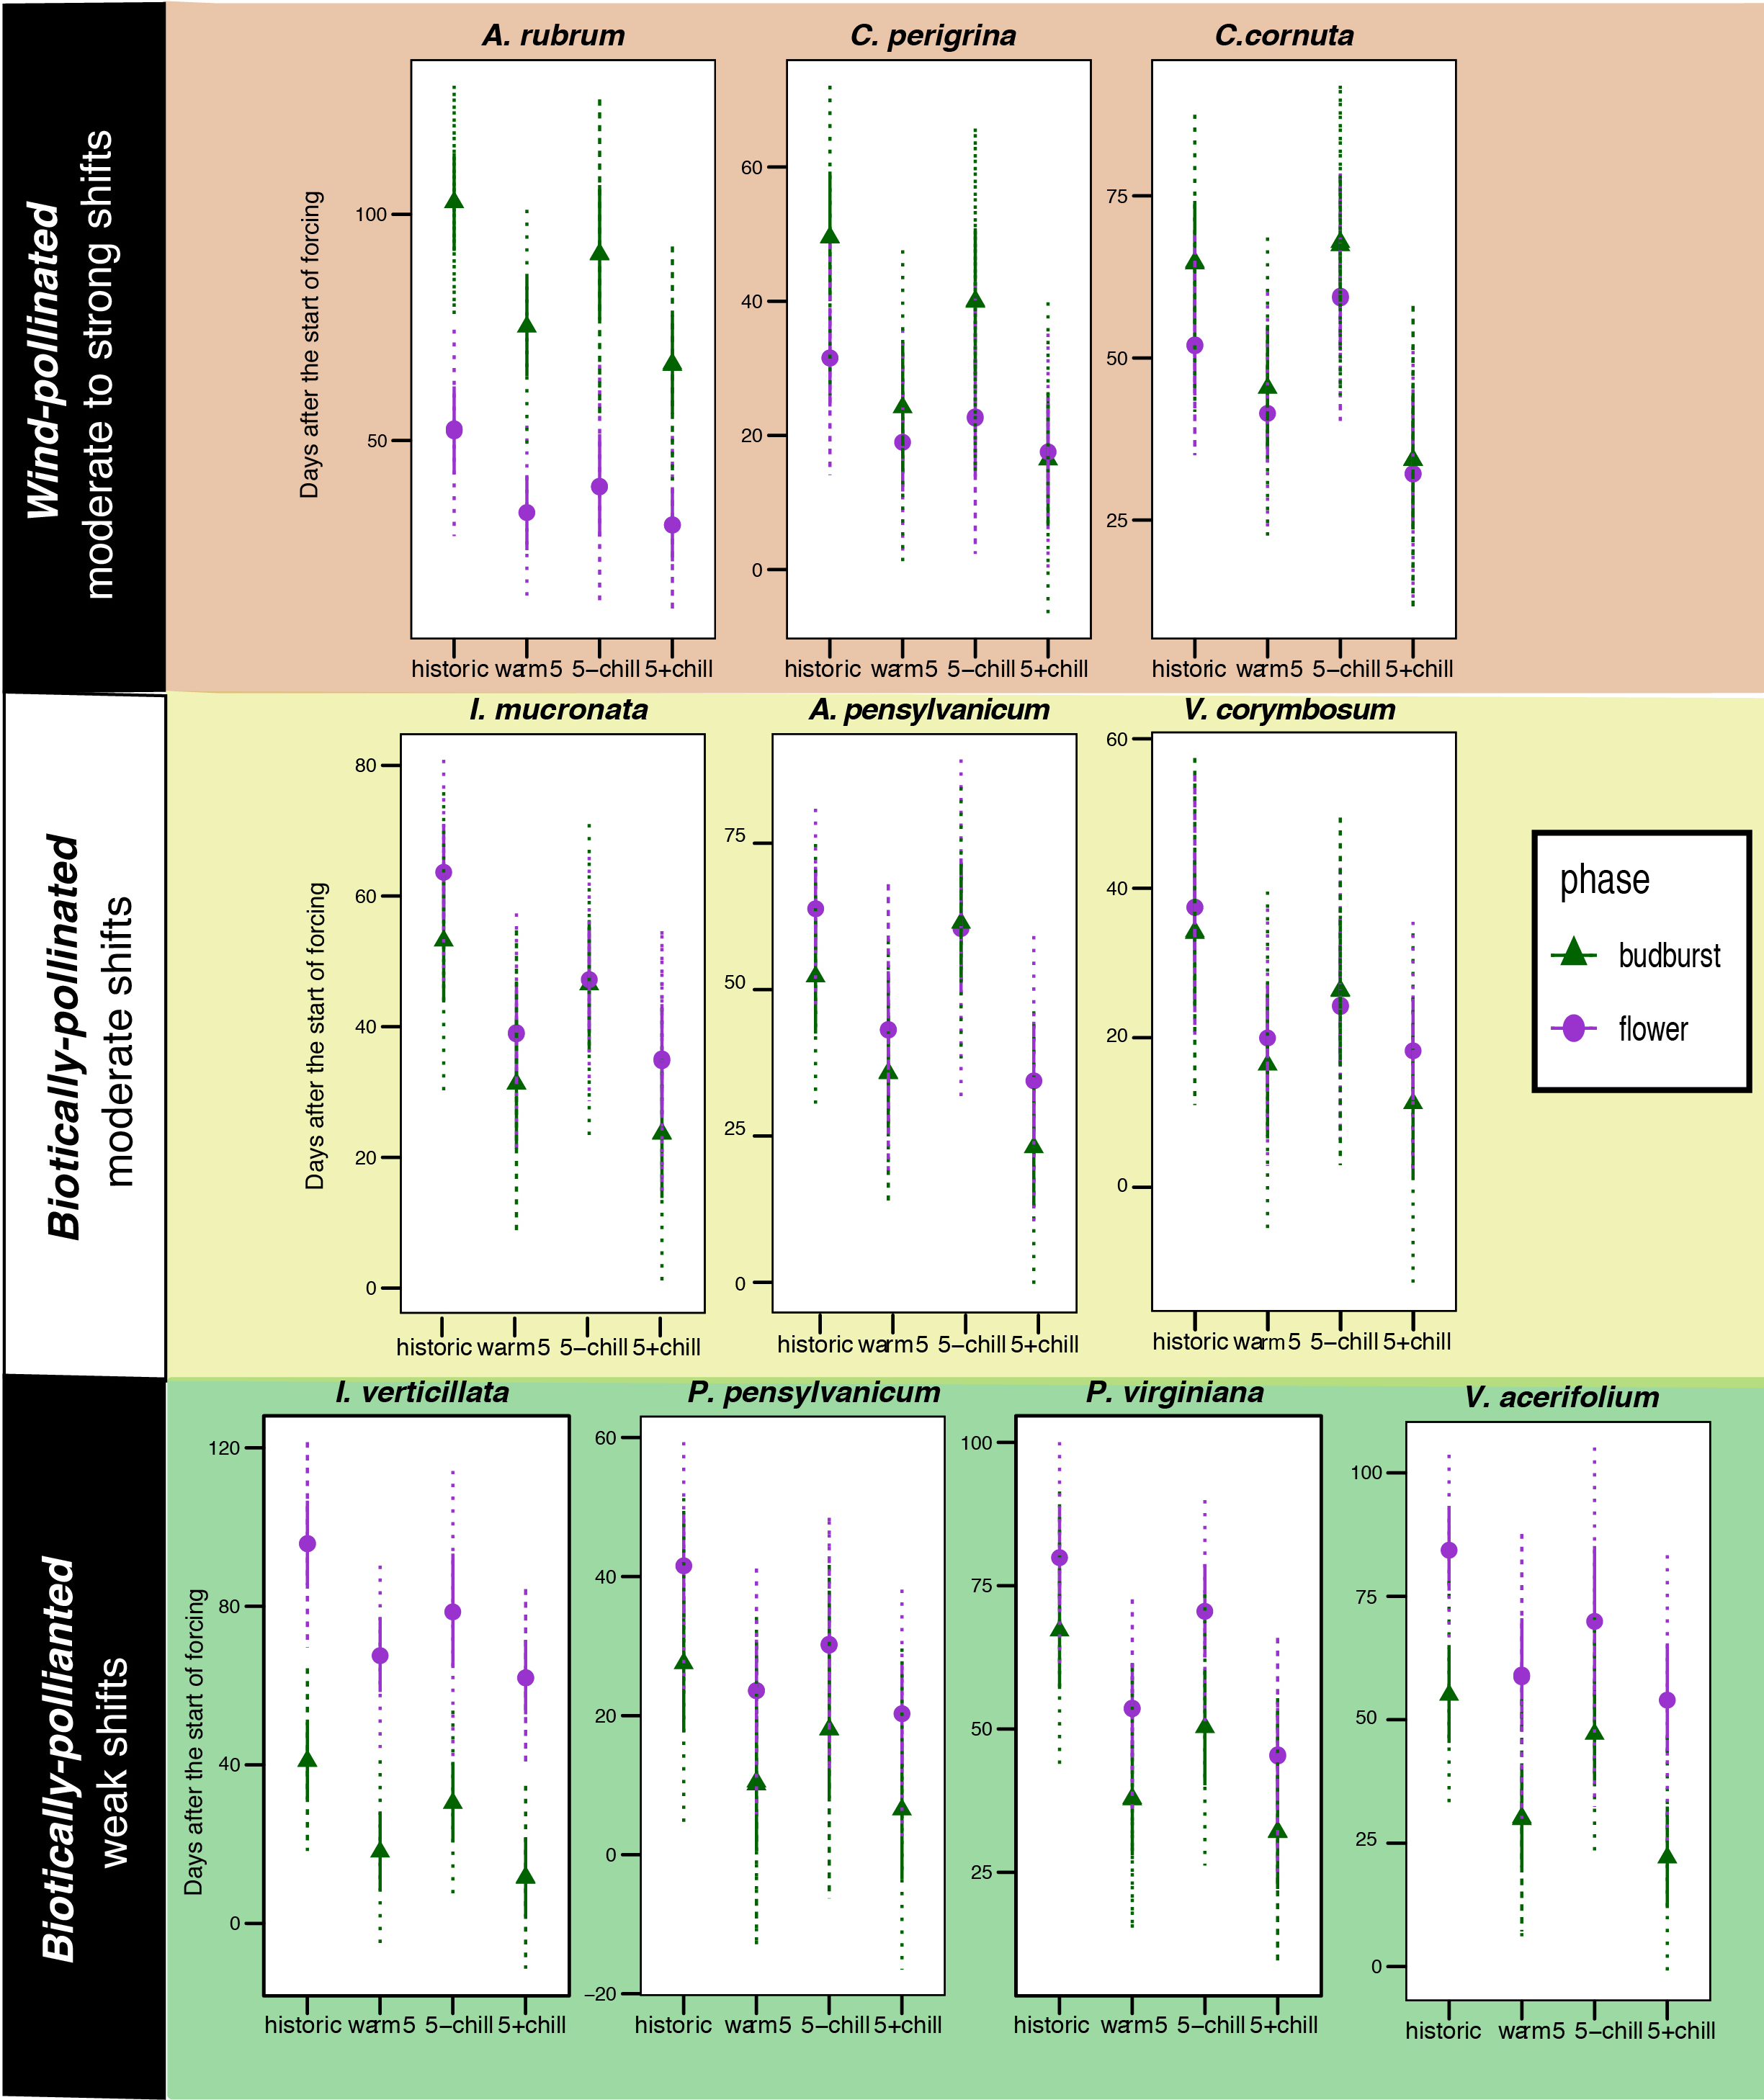
\includegraphics[width=\textwidth]{..//Plots/Flobuds_manuscript_figs/climpredictions.jpg}
    \caption{\textbf{Flower-leaf sequences (FLSs) of temperate, woody species will shift with climate change, but the magnitudes of these shifts vary by species and depend on the specific dynamics of temperature at a given location}. We used Bayesian, hierarchical models comparing flower and leaf bud responses to variable temperature combinations to predict FLSs patterns under current climate conditions and three climate change scenarios;  an increase in spring warming alone (warm 5), increase in spring warming and increase in winter chilling (warm 5 +chill) and an increase in spring warming and decrease in winter chill (warm 5 -chill). Projected FLS shifts are most pronounced in wind-pollinated, flowering-first species but FLS shifts for all species depend on the relationship between forcing and chilling changes which is likely to vary by location with climate change.}
    \label{fig:preddy}
\end{figure}


\end{document}